\begin{figure*}[ht!]
\centering
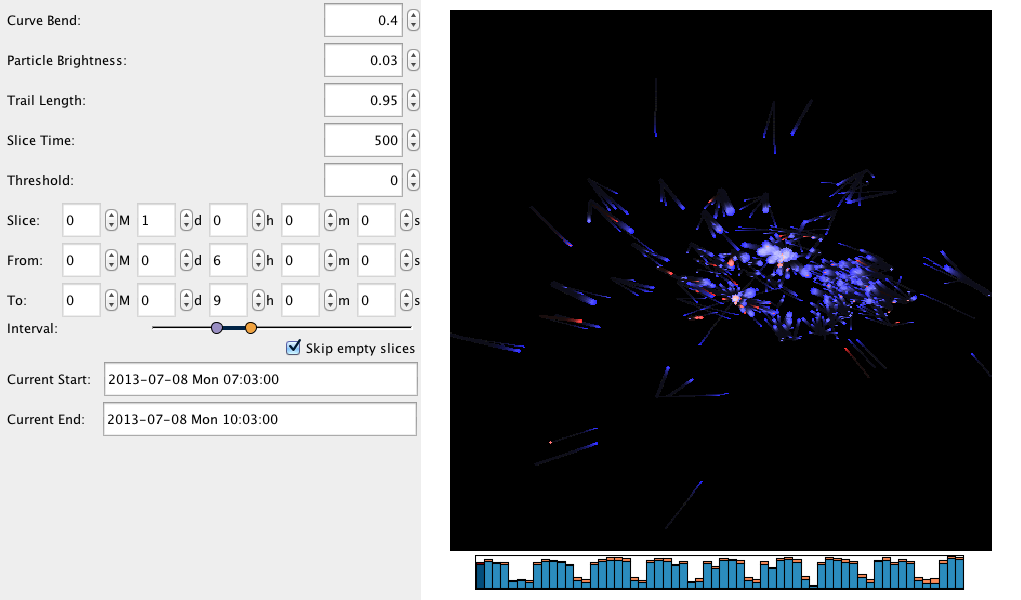
\includegraphics[width=0.9\linewidth]{images/tool.png}
\caption{The tool is split in three parts. On the right side is the
dot visualization. On the bottom right is the bar chart representation.
On the left is the control panel,
where the user can define the excursion of the trips, the brightness of
the dots, the length of the trails, the animation speed of the slices
and the threshold to remove dots that are too small.
With the spinners below this, the user can define the length of a slice and
the start and end of the relevant window.
The relevant window can also be edited by using the sliders below.
The user has also the option to skip slices that contain no trips, however
this only occurs when the duration of the slice is chosen very short.
The text fields at the bottom show the start and the end time of the
currently displayed relevant window.
}
\label{fig:tool}
\end{figure*}

\section{Data}
\label{sec:data}
The data used in this paper is provided by Capital~Bikeshare~\cite{wash}
the bike share company of Washington, DC. The data, reaching back
to October 2010, is freely available \cite{data}, though we used
only data from October 2012 until September 2013 to avoid the need
to skip the majority of the time to get to the latest data.
The remainder are 2470109 unique bicycle trips through Washington.

The trips are provided in multiple CSV files that vary in their format
per quarter.
Each trip consists of the name of the station where the bike was
picked up, the name of the station where the bike was put back, the time of
starting the trip, the duration, and whether the person was a
casual user or a subscribing member.
We processed the names of the stations,
usually consisting of the intersecting road names,
and converted them to geographic coordinates with a Geocoding
tool \cite{convert}.
We stored the trips in a MySQL database with the start time
as index to allow for fast ranged trip lookups by start time.
